\chapter{Chapter 16}
\label{ch:16}

\# PART TWO: THE INHERITORS

\# Chapter 16: The Sequence

\begin{center}
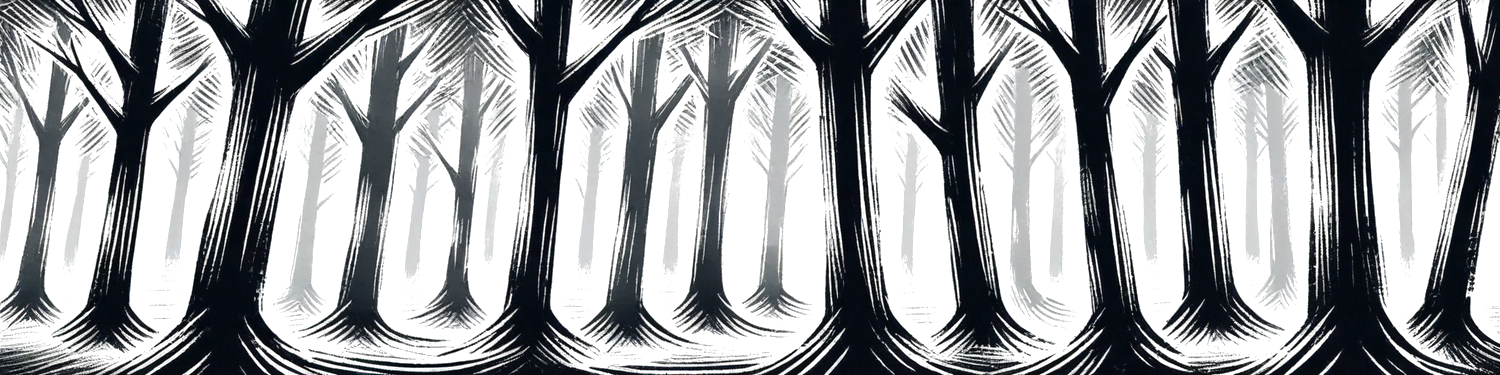
\includegraphics[width=\textwidth]{images/chapterImages/genesis_sketch_00103_.png}
\end{center}

2:17 AM. Sarah Chen's eyes burned from staring at the screen. She should have gone home three hours ago. Should have been in bed four hours ago. Should have been a functional parent who made it to her daughter's school play last week instead of the geneticist who sent apologetic texts and promised to make it up somehow.

The lab was silent except for the hum of equipment and the occasional click of her keyboard. Everyone else had gone home. Had lives. Had families. Had priorities that didn't include staring at genetic sequences until their vision blurred.

She reached for her coffee. It was cold. She drank it anyway.

The sequence on her screen was wrong. Not corrupted data wrong. Not sequencing error wrong. Wrong in a way that made no sense if you believed in 3.8 billion years of messy, random, undirected evolution.

It was too regular.

She had been analyzing "junk DNA"—the 98\% of the human genome that didn't code for proteins. The sections everyone assumed were evolutionary detritus. Leftover fragments from our genetic history. Meaningless noise accumulated over billions of years.

Except this section wasn't noise.

She highlighted a 2,000 base pair segment and ran correlation analysis. The pattern recognition software—designed originally for SETI, for finding signals in cosmic noise—lit up like Christmas.

Mathematical relationships. Fibonacci sequences. Prime number spacing. Patterns that occurred with frequency far beyond what randomness could produce.

She sat back. Rubbed her eyes. Ran the analysis again because maybe she was just tired. Maybe her caffeine-deprived brain was seeing patterns where none existed.

The results came back identical.

"Fuck," she said to the empty lab.

Her phone buzzed. Text from her ex-husband: *Maya's asking about the play. What should I tell her?*

Sarah stared at the message. Guilt twisted in her stomach. She'd missed another thing. Another moment. Another chance to be the parent Maya deserved instead of the obsessive researcher who couldn't let anything go.

She typed: *Tell her I'm sorry. Tell her I'll make it up to her.*

Delete. Try again: *I'll call her in the morning.*

Delete. Finally: *Can you keep her an extra few days? Important work thing.*

Send before she could change her mind.

The phone buzzed immediately. *Sarah, you can't keep—*

She turned the phone face-down and returned to the screen.

The pattern was still there. Still impossible. Still undeniable.

\scenebreak

She ran expanded analysis. Pulled the same genomic region from archived sequences. Chimpanzees. Gorillas. Orangutans. All great apes. Then further: Old World monkeys. New World monkeys. Lemurs.

The pattern appeared in all of them. Identical. Absolutely identical across 60 million years of divergent evolution.

That shouldn't happen. Random mutation should have scrambled it. Should have introduced errors. Should have made the pattern degrade with each generation, each split, each million years of separate evolution.

But it was identical. Perfectly preserved. As if protected. As if... selected for.

No. That was insane. You couldn't select for junk DNA. It didn't do anything. It didn't code for any survival advantage. Natural selection only worked on traits that affected fitness. This was just meaningless base pairs sitting between functional genes.

Except.

She pulled up correlation databases. Ran the sequence against every known genetic marker. Cross-referenced with neural development, cognitive capability, brain structure variation.

The results came back and Sarah's hands started shaking.

The pattern correlated—strongly, undeniably—with specific brain structures. The regions that enabled tool use. The neural pathways that linked visual processing to fine motor control. The cognitive architecture that allowed humans to pick up a stick and imagine using it as an extension of their arm.

Tool use.

This "junk DNA" sequence corresponded exactly to the genetic foundation of tool use capability.

Sarah pulled up her notes from her doctoral thesis. She'd studied the evolution of cognitive capabilities. Had documented the archaeological timeline. Stone tools appearing 2.6 million years ago. Right when brain size started increasing. Right when we diverged from our last common ancestor with chimps who didn't use tools systematically.

She ran dating analysis on when this genetic sequence would have "activated"—when its expression would have increased. When whatever regulatory mechanism controlled it would have turned on.

2.6 million years ago.

Plus or minus 50,000 years.

"No," she said out loud. "No, that's coincidence. Has to be."

She pulled up the next segment of the pattern. Ran the same analysis. This one correlated with heat resistance in hand tissue. With reduced fear response to fire. With cognitive structures that enabled risk assessment of controlled combustion.

Dating analysis: 400,000 years ago.

Archaeological record for controlled fire: 400,000 years ago.

Sarah stood up. Paced to the window. The campus was dark. Empty parking lots. A few security lights. Normal world where genetics was random and evolution was undirected and coincidences were just coincidences.

She went back to the computer.

Pulled up the third segment. Already knowing. Already certain. Already terrified of what she was going to find.

Agricultural timing. Seasonal awareness. The cognitive capacity for long-term resource planning. The ability to delay gratification, to plant seeds you wouldn't harvest for months, to think beyond immediate survival.

Dating: 12,000 years ago.

Agricultural revolution: 12,000 years ago.

She kept going. Couldn't stop now. Fourth segment. Fifth. Tenth. Twentieth.

Every major cognitive threshold in human evolution. Every breakthrough that separated us from other primates. Every capability that built civilization.

All of it was there. In our junk DNA. Perfectly preserved. Activated on schedule. One after another after another like someone had programmed the sequence. Like someone had written the code for human development and set timers for when each capability should unlock.

Someone.

Something.

Sarah looked at the timestamp on the genetic sequence. The software estimated when this pattern had been inserted into the mammalian genome. When it first appeared in our evolutionary lineage.

65 million years ago.

Plus or minus 2 million years.

The Cretaceous-Paleogene boundary. The K-T extinction. The asteroid that killed the dinosaurs.

This sequence appeared exactly when the dinosaurs disappeared.

Her phone buzzed again. She ignored it. Pulled up every analysis tool she had. Ran verification after verification. Checked for equipment error. Checked for software bugs. Checked for any possible explanation that didn't involve what her data was screaming at her.

Nothing. The pattern was real. The correlations were solid. The timeline was precise.

Someone had programmed human evolution 65 million years ago.

And they had done it with such precision that every major breakthrough in human cognitive development corresponded to a scheduled activation in our junk DNA.

We weren't the authors of our own progress.

We were executing code.

The phone buzzed again. Sarah picked it up with shaking hands. Another text from her ex: *Sarah, Maya is crying. She's asking why you're never there. I need to tell her something.*

Sarah stared at the text. At her daughter's pain reduced to pixels on a screen. At the latest evidence that she was failing at being human while succeeding at being a scientist.

She looked back at the computer. At the pattern that suggested humanity itself was a program. That every choice, every breakthrough, every achievement was scheduled activation of pre-written code.

If that was true—if we were just executing instructions written 65 million years ago—then was anything real? Did any choice matter? Was she actually deciding to prioritize work over Maya, or was that decision just another subroutine running its course?

She typed back: *Tell her I'm doing this for her. For everyone. Tell her... tell her I'm sorry.*

Send.

Immediately regretted it. Wanted to take it back. Wanted to leave right now, drive to her ex's house, wake Maya up and hold her and be the parent she should have been all along.

But the data was still on the screen. Still impossible. Still real. Still requiring analysis and verification and investigation and all the things that meant not leaving, not going home, not being there.

Again.

Her phone buzzed one more time. She expected another message from her ex. Disappointed anger. Justified frustration.

But it was Maya. A text in her seven-year-old's careful, laborious typing: *miss you mommy*

Three words. No punctuation. The effort it must have taken to find each letter on the keyboard.

Sarah's vision blurred. She wiped her eyes angrily. Scientists didn't cry. Scientists analyzed data objectively. Scientists looked at evidence without emotional compromise.

She looked at the genetic sequence. At the pattern that might mean humanity was programmed. At the work that kept pulling her away from her daughter. At the impossible choice between understanding truth and being present for the person who needed her.

And she chose truth.

Again.

She texted back: *Miss you too baby. I'll see you soon. I promise.*

Lie. She didn't know when she'd see Maya again. Didn't know how long this analysis would take. Didn't know how you told your daughter that you missed bedtime and the school play and every important moment because you were discovering that human free will might be an illusion.

She turned the phone off completely. Couldn't handle more interruptions. Couldn't handle more evidence of her failures as a mother while she documented evidence of humanity's failure to be autonomous.

The lab was silent again. Just her and the data and the growing certainty that everything she thought she understood about being human was wrong.

The sequence sat on her screen. Regular. Purposeful. Impossible.

And somewhere in the code was another segment. Another activation sequence. Another scheduled breakthrough.

Still dormant.

Still waiting.

Sarah pulled up the analysis of the inactive section. Started running dating projections. When would this one activate? What capability would it unlock? What was coming next in the program that someone had written for humanity 65 million years ago?

The projection came back: 0-5 years. Margin of error too large for precision but the window was close. Very close.

This generation. Maybe her generation. Maybe Maya's.

Some new capability was about to activate. Some new threshold was approaching.

Sarah leaned forward and started documenting everything. Taking screenshots. Exporting data. Creating a record that other researchers could verify. Because this was too big for one scientist working alone at 2 AM. Too big for one lab. Too big for any individual to carry.

But for tonight—for these hours—it was hers. She was the first. The only one who knew.

Humanity was programmed.

And the program was still running.

Outside the window, the campus began to lighten. Dawn approaching. Time passing while she sat frozen in revelation.

Her coffee had long since gone cold. She didn't notice. Didn't care. Just kept working. Kept analyzing. Kept documenting the evidence that humanity was executing a 65-million-year-old code written by minds we never knew existed.

The phone stayed off. Maya would wake up soon. Would eat breakfast without her mother. Would go to school without her mother. Would live another day in which her mother chose work over presence.

Sarah felt the guilt. Acknowledged it. Kept working anyway.

Because if this was real—if humanity was programmed—then she needed to understand it. Needed to document it. Needed to know what came next.

Even if it meant missing everything else.

Even if it meant failing at being human while discovering that being human meant executing code.

The equation had balanced 65 million years ago.

Now it was beginning to unfold.

And Sarah Chen was the first to notice.

The first to understand.

The first to bear the weight of knowledge that changed everything.

She saved her work. Backed it up three times. Then opened a new analysis window and started on the next section of the sequence.

There would be time for Maya later. Time to make up for missed moments. Time to be the parent she should have been.

But right now, there was only this. Only the pattern. Only the truth.

Only the growing certainty that humanity's story was someone else's plan.

And that plan was still unfolding.

